\section{Background}\label{sec:background}

%Give a short, self-contained summary of necessary
%background information. For example, assume you present an
%implementation of FFT algorithms. You could organize into DFT
%definition, FFTs considered, and cost analysis. The goal of the
%background section is to make the paper self-contained for an audience
%as large as possible. As in every section
%you start with a very brief overview of the section. Here it could be as follows: In this section 
%we formally define the discrete Fourier transform, introduce the algorithms we use
%and perform a cost analysis.

\mypar{Belief Propagation}
Belief Propagation (BP) is a technique in the domain of machine learning to perform probabilistic inference on graphical models, out of which Bayesian Networks and Markov Random Fields are the most well known. The standard version of BP is designed to deal with factor graphs, a bipartite graph that can represent Bayesian Networks or Markov Random Fields. Each node of the factor graphs represents the state of a random variable. Through message passing the state of the nodes is inferred. BP, also known as sum-product algorithm, computes the message sent from node $v_i$ to $v_j$ using equation \ref{eqn:bp_message}.
\begin{equation}                                                            
\label{eqn:bp_message}
m_{ij}(x_c) = \sum_{x_d \in X}\phi_i(x_d)\psi_{ij}(x_d,x_c)\prod_{k \in N(i) \ j}m_{ki}(x_d)
\end{equation}

\textbf{TODO: describe formula, add loopy etc.} \\


\mypar{Top-N Recommendation}
Top-N Recommendation is the problem where for a user $u_i$ one generates a list of n recommended objects, in our case movies, using a list of ratings by this and other users. Ha et al. \cite{Ha:2012:TRT:2396761.2398636} propose a method for top-n recommendation using loopy belief propagation. The factor graph for top-n recommendation consists of nodes for the users and movies. To predict $u_i$s top movies a factor graph is created. The graph consists of all users and movies. For every rating by $u_i$ a factor is created and the user, movie and factor are connected. The ratings of the other users are only added if the rating exceeds a certain threshold. Each user and movie node is initialized with the likelihood whether user $u_i$ likes the node or not. Figure \ref{top_n_graph} shows a small factor graph for user $i=2$ where user $u1$ has rated the movies $m1,m2$, $u2$ the movie $m2$ and $u3$ the movies $m1,m2$ and $m3$. Initially it is only known, that user $u_2$ likes the movie $m_2$ with a probability of 0.7. All other nodes are initialized with a probability of 0.5 for like and 0.5 for don't like. A rating of 5 (best) sets the like probability to 0.9 whereas the rating 1 (worst) sets the probability to 0.1. The probabilities for ratings in between are interpolated. \textbf{TODO: erwaehnen, dass nodes in anderen Anwendungen mehr als nur zwei states haben koennten?}
Using loopy belief propagation the most important messages are sent through the factors and the belief is propagated from observed nodes to unobserved nodes (see Figure \ref{top_n_graph_important_msg}). When the belief propagation converges each movie has a probability "User $i$ likes movie $j$". Figure \ref{top_n_graph_final_state} shows a possible final state. The movies can be sorted and the top N elements are returned. In this example Movie $m_1$ would be the top-one recommendation for user $u_2$.

\begin{figure}[h]\centering
    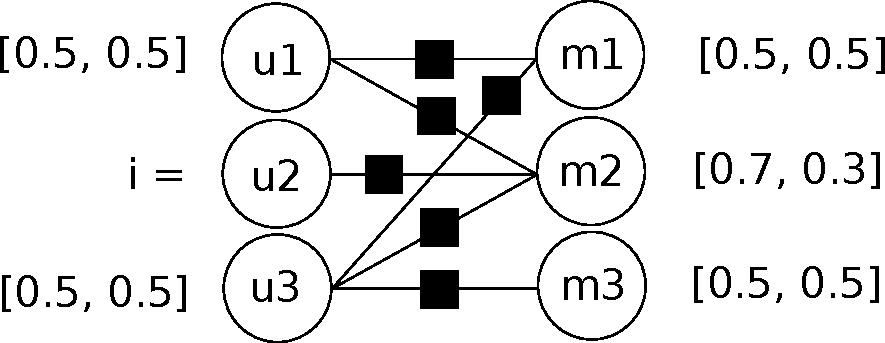
\includegraphics[scale=0.33]{graphics/top-n-graph.pdf}
  \caption{Factor Graph for predicting top-n movies for user $u_2$. The dark squares are the factors. The values in [] show the probabilities for the random variables being in state "like" or "don't like".\label{top_n_graph}}
\end{figure}

\begin{figure}[h]\centering
    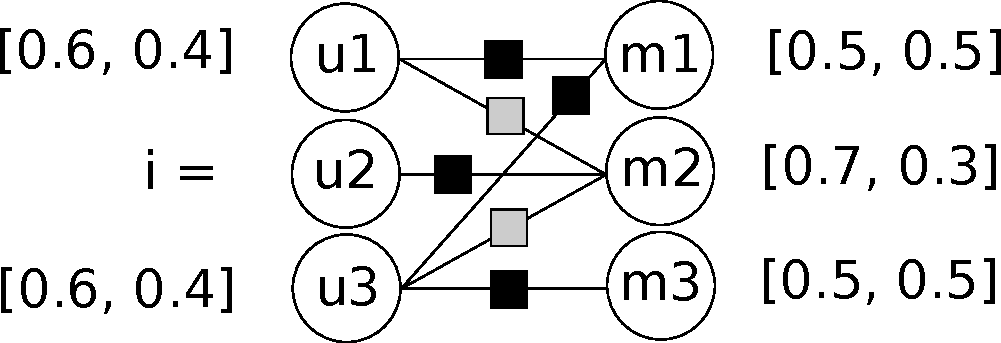
\includegraphics[scale=0.33]{graphics/top-n-important-messages.pdf}
  \caption{Belief is propagated from observed node $m_2$ to unobserved notes \label{top_n_graph_important_msg}}
\end{figure}

\begin{figure}[h]\centering
    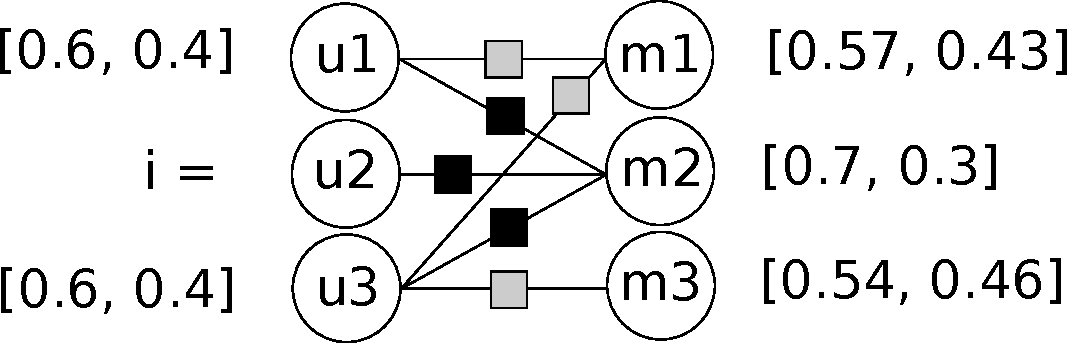
\includegraphics[scale=0.33]{graphics/top-n-final.pdf}
  \caption{A possible final state for top-n recommendation. Movie $m_1$ is the top recommendation for user $u_2$. \label{top_n_graph_final_state}}
\end{figure}


\mypar{Cost Analysis}
\textbf{TODO}

%\mypar{Discrete Fourier Transform}
%Precisely define the transform so I understand it even if I have never
%seen it before.
%
%\mypar{Fast Fourier Transforms}
%Explain the algorithm you use.
%
%\mypar{Cost Analysis}
%First define you cost measure (what you count) and then compute the
%cost. Ideally precisely, at least asymptotically. In the latter case you will need to instrument your code to count
%the operations so you can create a performance plot.
%
%Also state what is
%known about the complexity (asymptotic usually) 
%about your problem (including citations).